%	
%	disposition.tex
%	
%	This document provides a summary of all of the exam question topics for
%	the algorithms and datastructures course at the university of copenhagen
%	department of computer science. It was written to serve as an excellent
%	asset for the oral exam preparation, with most of the subtopics covered
%	for any given exam topic in a concise and easily understandable format.
%	

\documentclass[11pt,english]{book}

\usepackage{appendix}						% appendices
\usepackage[linesnumbered]{algorithm2e}		% algorithm pseudo-code
\usepackage{amsthm,amsmath,amssymb}			% mathematical notation
\usepackage{fancyhdr}						% page styling
\usepackage{float}							% for floating figures
\usepackage{sectsty}						% section styling
\usepackage{tikz} 							% for graphs

%========== meta data ==========%

\title
{
	Algorithms \& Datastructures\\
	\huge Disposition
}

\author
{
	Casper B. Hansen\\
	\small Department of Computer Science\\
	\small The University of Copenhagen\\
	\texttt{fvx507@alumni.ku.dk}
% fix this, makes footnote number, and it shouldn't!
%	\thanks{Adam Honoré}
%	\thanks{Mads Torhus}
}


\date{\today}


%========== settings ==========%

\setlength{\headheight}{15pt}
\sectionfont{\Large}


%========== macros ==========%

\newcommand{\sethead}[3]{\lhead{#1}\chead{#2}\rhead{#3}}
\newcommand{\setfeet}[3]{\lfoot{#1}\cfoot{#2}\rfoot{#3}}

\newtheorem{theorem}{Theorem}[section]
\newtheorem{lemma}[theorem]{Lemma}
\newtheorem{proposition}[theorem]{Proposition}
\newtheorem{corollary}[theorem]{Corollary}

% \newenvironment{proof}[1][Proof]{\begin{trivlist}
% \item[\hskip \labelsep {\bfseries #1}]}{\end{trivlist}}
\newenvironment{definition}[1][Definition]{\begin{trivlist}
\item[\hskip \labelsep {\bfseries #1}]}{\end{trivlist}}
\newenvironment{example}[1][Example]{\begin{trivlist}
\item[\hskip \labelsep {\bfseries #1}]}{\end{trivlist}}
\newenvironment{remark}[1][Remark]{\begin{trivlist}
\item[\hskip \labelsep {\bfseries #1}]}{\end{trivlist}}

% \newcommand{\qed}{\nobreak \ifvmode \relax \else
%      \ifdim\lastskip<1.5em \hskip-\lastskip
%      \hskip1.5em plus0em minus0.5em \fi \nobreak
%      \vrule height0.75em width0.5em depth0.25em\fi}

%========== document ==========%

\begin{document}

\frontmatter
\maketitle
\thispagestyle{empty}
\tableofcontents

%========== preamble ==========%

\newpage
\pagestyle{fancy}

\chapter*{Preamble}
In this document we will discuss the most important principles of algorithms
and datastructures in accordance with the syllabus of the course under the
same title at the University of Copenhagen, Department of Computer Science.

\section*{About the authors}
We're a small group of Computer Science students, attending the course
mentioned above at the time of writing this document as collaborative effort
to make a great disposition for the course exam, that will both increase our
own understanding of the subjects discussed as well as produce an invaluable
resource for others attending the course, or who wish to learn about
algorithms and datastructures in generel.

\section*{Why we made this document}
The document is was written in order to support our own understanding of the
course contents as well as aid us during the exam preparation time.

\section*{How to use this document}
The intention of the document is \textit{not} to be a fullfledged introduction
to algorithms and datastructure that you can just pick up and start learning
from. As such it requires at least an accompanying book, or that you are
attending lectures on the subject, or some other means that provide a base
knowledge.

The document is merely a tool for looking up things quickly, and defines the
subjects in a concise manner, hence no in-depth discussion of any subject is
to be found in this document. The sole purpose of the document is precisely
that; a resource for quickly looking up the concepts discussed presented at
lectures, or in a book.

\section*{Recommendations}
As far as we know the book \textit{Introduction to Algorithms} by Thomas H.
Cormen, Charles E. Leiserson, Ronald L. Rivest and Clifford Stein, is pretty
much the go-to choice if you want to study algorithms, and since this was our
textbook during the course this is what we'll recommend for you.



\mainmatter
%========== Divide & Conquer ==========%

\chapter{Divide \& Conquer}
\label{ch:divideandconquer}

\textbf{Assignments} 2-2 (counter example), 7-1 (quicksort)\\\\
\textbf{Pensum} 2.3 + 4 + 7 \cite{clrs} \\\\
\textbf{Algorithms} Merge sort, quicksort, fibonacci\\\\
\textbf{Keywords} Recurrences, master method
\vspace{1in}

\noindent Divide and conquer is a paradigm of algorithmic methodologies. It
takes a problem and \textit{divides} it into several smaller subproblems,
until it reaches a base case, which makes the algorithm \textit{bottom out},
or \textit{conquer} each of these subproblems. \textit{Combining} the
solutions of all of the subproblems then yields a correct solution to the
original problem.
\\\\
\noindent \textbf{Divide} the problem into a number of subproblems that are
smaller instances of the same problem.
\\\\
\noindent \textbf{Conquer} the subproblems by solving them recursively. If the
subproblem sizes are small enough, however, just solve the subproblems
trivially.
\\\\
\noindent \textbf{Combine} the solutions to the subproblems into the solution
for the original problem.
\\\\

\section{Solving Recurrences}
% p. 83-97, CLRS 
Divide and conquer algorithms give rise to recurrence naturally, because they
call themselves recursively. To analyze the complexity of any recursive
algorithm we must describe it mathematically as an equation or inequality.
\\\\
We do this using one of three methods.
\begin{description}
	\item \textbf{Recursion trees} describes the recursions by means of a
tree-structure, by which we can then either guess or argue the complexity.
	\item \textbf{Substitution} uses a guessed bound, which could have been
derived from a recursion tree, and then by mathematical induction proves this
bound.
	\item \textbf{Master method} provides formulae for recurrences of the form
$T(n) = a T(n/b) + f(n)$, where $a \geq 1$, $b > 1$ and $f(n)$ is a given
function.
\end{description}

\subsection{Recursion Trees}
% p. 88-92, CLRS
A recursion tree is a pictorial representation of an algorithms recursive
calls. That is, we simply draw the recursions as they occur in a
tree-structure, such that we may make a guess as to the complexity of an
algorithm.

\begin{figure}[h]
	\center
	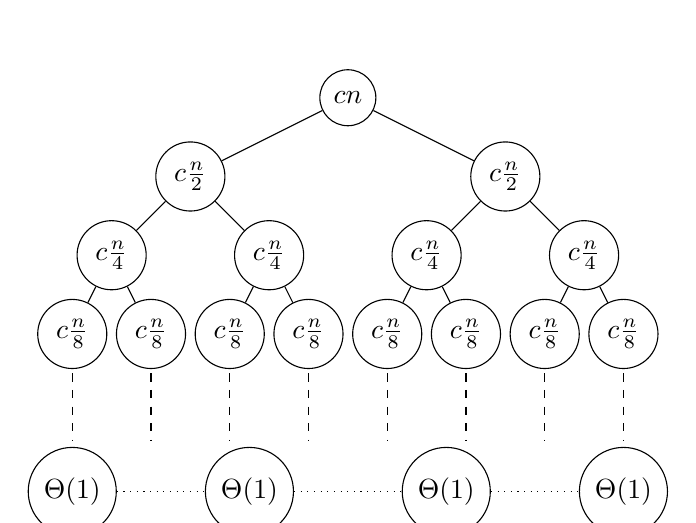
\begin{tikzpicture}
	[
	scale=1.0,
	align=center,
	every node/.style={circle, fill=white, draw=black}
	]
		% level 1
		\node (n1) at 	(3.5, -1) {$cn$};
		
		% level 2
		\node (n2) at 	(1.5, -2) {$c\frac{n}{2}$};
		\node (n3) at 	(5.5, -2) {$c\frac{n}{2}$};
		
		% level 3
		\node (n4) at 	(0.5, -3) {$c\frac{n}{4}$};
		\node (n5) at 	(2.5, -3) {$c\frac{n}{4}$};
		\node (n6) at 	(4.5, -3) {$c\frac{n}{4}$};
		\node (n7) at 	(6.5, -3) {$c\frac{n}{4}$};
		
		% level 4
		\node (n8) at 	(0, -4) {$c\frac{n}{8}$};
		\node (n9) at 	(1, -4) {$c\frac{n}{8}$};
		\node (n10) at 	(2, -4) {$c\frac{n}{8}$};
		\node (n11) at 	(3, -4) {$c\frac{n}{8}$};
		\node (n12) at 	(4, -4) {$c\frac{n}{8}$};
		\node (n13) at 	(5, -4) {$c\frac{n}{8}$};
		\node (n14) at 	(6, -4) {$c\frac{n}{8}$};
		\node (n15) at 	(7, -4) {$c\frac{n}{8}$};
		
		% bottom-out level
		\node (l1) at (0, -6) {$\Theta(1)$};
		\node (l2) at (2.25, -6) {$\Theta(1)$};
		\node (l3) at (4.75, -6) {$\Theta(1)$};
		\node (l4) at (7, -6) {$\Theta(1)$};
		
		% drawing code
		\draw [dashed] (0, -4.5) -- (0, -5.35);
		\draw [dashed] (1, -4.5) -- (1, -5.35);
		\draw [dashed] (2, -4.5) -- (2, -5.35);
		\draw [dashed] (3, -4.5) -- (3, -5.35);
		\draw [dashed] (4, -4.5) -- (4, -5.35);
		\draw [dashed] (5, -4.5) -- (5, -5.35);
		\draw [dashed] (6, -4.5) -- (6, -5.35);
		\draw [dashed] (7, -4.5) -- (7, -5.35);
		\foreach \from/\to in {n1/n2,n1/n3} \draw (\from) -- (\to);
		\foreach \from/\to in {n2/n4,n2/n5,n3/n6,n3/n7} \draw (\from) -- (\to);
		\foreach \from/\to in {n4/n8,n4/n9,n5/n10,n5/n11,n6/n12,n6/n13,n7/n14,n7/n15} \draw (\from) -- (\to);
		\foreach \from/\to in {l1/l2,l2/l3,l3/l4} \draw [dotted] (\from) -- (\to);
	\end{tikzpicture}

	\caption{Recurrence tree of merge sort.}
\end{figure}

Although recursion trees are useful for getting an idea about the complexity
of a recursive algorithm, it doesn't directly give us any concrete about this.
For that must employ more strict methods that are rooted in mathematics, and
not drawings - we can do this by induction with the substitution method (see
section \ref{ch:divideandconquer|sub:recurrences|subsub:substitution}).

\subsection{Substitution}
\label{ch:divideandconquer|sub:recurrences|subsub:substitution}
% p. 83-87, CLRS
The substitution method for solving recurrences consists of
two steps:
\begin{itemize}
\item Guess the form of the solution.
\item Use mathematical induction to find constants in the form and show that
the solution works.
\end{itemize}
The inductive hypothesis is applied to smaller values,
similar like recursive calls bring us closer to the base case
\\\\
\noindent \textbf{Example}\\
The recurrence relation for the cost of a divide-and-conquer method is
$T(n) = 2T( \lfloor n/2 \rfloor ) + n$. Our induction hypothesis of $T(n)$ is
$O(n \lg n)$ or $T(n) \leq cn \lg n$ for some constant $c$, independent of $n$.

Assume the hypothesis holds for all $m < n$ and substitute:
\begin{align}
	T(n) &\leq 2(c \lfloor n/2 \rfloor \lg_2 (\lfloor n/2 \rfloor )) + n \\
	&\leq cn \lg_2(n/2)+n \\
	&= cn \lg_2(n) - cn \lg_2(2)+n \\
	&= cn \lg_2(n) - cn + n \\
	&\leq cn \lg_2 (n)
\end{align}
as long as $c \geq 1$.

\newpage
\subsection{The Master Method}
\label{ch:divideandconquer|sub:recurrences|sub:master-theorem}
% p. 88-97, CLRS
For a divide-and-conquer algorithm $T(n)$, let $a$ denote the number of
subproblems created, and $n/b$ denote the size of each of these, on each
recursion. For each recursion we have a combine step, which takes $f(n)$.
We then have a recurrence of the form $T(n) = a T(n/b) + f(n)$.

Algorithms of this form can be solved by means of the master theorem, which
is given by
\begin{align}
\label{eqn:master-theorem}
	T(n) &= a T\left(\frac{n}{b}\right) + f(n)
	\begin{cases}
		f(n) = O(n^{\lg_b a - \epsilon}) & T(n) = \Theta(n^{\lg_b a}) \\
		f(n) = \Theta(n^{\lg_b a}) & T(n) = \Theta(n^{\lg_b a} \lg n) \\
		f(n) = O(n^{\lg_b a + \epsilon}) & * \Rightarrow T(n) = \Theta(f(n))
	\end{cases}
\end{align}
where $a \geq 1$, $b > 1$ and $\epsilon > 0$.
\begin{align}
	a f\left(\frac{n}{b}\right) &\leq c f(n)
	\text{, for all sufficiently large } n \text{, where } c < 1 \tag{*}
\end{align}
The first case $O(n^{\lg_b a - \epsilon})$ occurs when the \textit{divide}
step of the algorithm contributes the most to the complexity of the algorithm,
since $n^{\lg_b a} > f(n)$, and we therefore have to account for this by
subtracting $\epsilon$ from the exponent on the left-hand side. Vice versa for
the third case $O(n^{\lg_b a + \epsilon})$, which is symmetric. The second
case $\Theta(n^{\lg_b a})$ occurs when both steps, the \textit{divide} and
\textit{combine} step, are of the same complexity.
\\\\
\noindent \textbf{Example} \\
Consider the recurrence $T(n) = 2T(n/2) + f(n)$ of merge sort. We identify the
variables values as $a = 2$ since each recursive call creates two subproblems
and $b = 2$ since each of these are of $n/2$ the size of the previous problem.
The combine step is of linear time $\Theta(n)$.

We then have that $O(n^{\lg_2 2}) = f(n)$, since $f(n) = \Theta(n)$ and this
satisfies the previous equation, because $O(n^{\lg_2 2}) = \Theta(n)$.
Therefore, the second case of the master theorem applies to this algorithm,
and the complexity of it is then $\Theta(n^{lg_2 2}\lg n) = \Theta(n \lg n)$.





%========== Heaps ==========%

\chapter{Heaps}
\label{ch:heaps}

\textbf{Pensum} 6 \cite{clrs} \\\\
\textbf{Assignments} 2-2 (counter example), 13-3 (tree relation) \\\\
\textbf{Algorithms} Heap-sort \\\\
\textbf{Keywords} Min- and maxheap, sorting, priority queues
\vspace{1in}

\noindent A heap is a nearly complete $n$-nary tree, we will concern ourselves
only with binary heaps - and as such, a binary heap is a nearly complete
binary tree. A heap implements a set $S$ of elements, in which each element
has an associated key. The actual structure of a heap is simply an array, and
so a heap is defined by the operations performed on the array, rather than the
data structure itself. The reason a heap is a tree-structure is a
visualization of the data, but not reflected by the data structure in any way.

Visualizing the array of a heap as a tree, we have that the root of the tree
corresponds to the first element of the array $i = 0$ (zero-indexed). The
parent of any node $n$ is given by $\lfloor n/2 \rfloor$. The children are
given by $2n$ and $2n + 1$, for left and right, respectively.

\newpage
\noindent Using the rules of traversal defined above, we can visualize the
array
\begin{figure}[H]
	\center
	\begin{tabular}{|c|c|c|c|c|c|c|c|c|c|}
		\hline 16 & 14 & 10 & 8 & 7 & 9 & 3 & 2 & 4 & 1 \\ \hline
	\end{tabular}
	\caption{Example of a (binary-)heap}
	\label{fig:heap-array}
\end{figure}
as a tree-structure, as shown in the following figure.
\begin{figure}[H]
	\center
	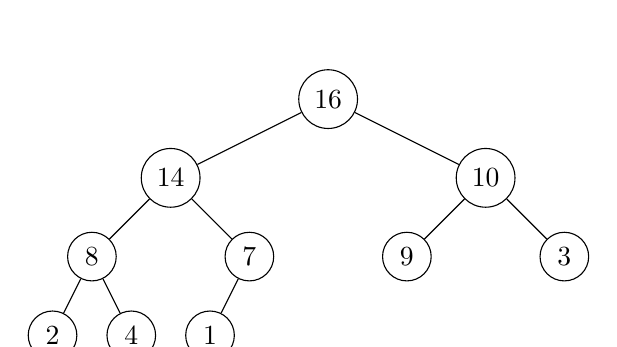
\begin{tikzpicture}
	[
	scale=1.0,
	align=center,
	every node/.style={circle, fill=white, draw=black}
	]
		% level 1
		\node (n1) at 	(3.5, -1) {16};

		% level 2
		\node (n2) at 	(1.5, -2) {14};
		\node (n3) at 	(5.5, -2) {10};

		% level 3
		\node (n4) at 	(0.5, -3) {8};
		\node (n5) at 	(2.5, -3) {7};
		\node (n6) at 	(4.5, -3) {9};
		\node (n7) at 	(6.5, -3) {3};

		% level 4
		\node (n8) at 	(0, -4) {2};
		\node (n9) at 	(1, -4) {4};
		\node (n10) at 	(2, -4) {1};
		% \node (n11) at 	(3, -4) {11};
		% \node (n12) at 	(4, -4) {12};
		% \node (n13) at 	(5, -4) {13};
		% \node (n14) at 	(6, -4) {14};
		% \node (n15) at 	(7, -4) {15};

		% drawing code
		\foreach \from/\to in {n1/n2,n1/n3} \draw (\from) -- (\to);
		\foreach \from/\to in {n2/n4,n2/n5,n3/n6,n3/n7} \draw (\from) -- (\to);
		\foreach \from/\to in {n4/n8,n4/n9,n5/n10} \draw (\from) -- (\to);
	\end{tikzpicture}
	\caption{Example of a (binary-)heap visualized as a tree}
	\label{fig:heap-tree}
\end{figure}

\section{Priority Queues}
\label{ch:heaps|sub:priorityqueues}
A priority queue is an abstract data structure, which sorts and maintains a
set of data in such a way, that the data is prioritized.A priority queue is not a destinct structure but a
class of data structures. Priority queues work well with stacks, heaps, self-organizing lists, etc. We will focus
mainly on heaps.
A heap is a priority queue and must adhere to the properties of either max or min-heap.
\begin{description}
	\item \textbf{Max-heap} The key of a node is greater than or equal to the
keys of its children.
	\item \textbf{Min-heap} The key of a node is less than or equal to the
keys of its children.
\end{description}
Max- and Min-Heaps are defined by their procedures, and we must show that their properties are maintained by those.

\clearpage

\begin{algorithm}[H]
	\caption{Max-heapify}
	\label{alg:max-heapify}

	\SetKwInOut{Input}{Input}
	\SetKwInOut{Output}{Output}

	\SetKwFunction{MaxHeapify}{MaxHeapify}
	\SetKwFunction{Left}{Left}
	\SetKwFunction{Right}{Right}

	\Input{An array $A$ and index $i$}
	\Output{In-place swapping max-heap property violations of $A$.}

	\BlankLine
	\MaxHeapify($A$, $i$) \\
	\Begin
	{
		$l = $ \Left($i$) \\
		$r = $ \Right($i$) \\
		$largest = i$ \\
		\If{$l \leq A.size $ \textnormal{and} $A[l] > A[i]$}
		{
			$largest = l$ \\
		}
		\If{$r \leq A.size $ \textnormal{and} $A[r] > A[largest]$}
		{
			$largest = r$ \\
		}
		\If{$largest \neq i$}
		{
			Swap $A[i]$ and $A[largest]$ \\
			\MaxHeapify($A$, $largest$)
		}
	}
\end{algorithm}
The procedure looks for a violation of the max-heap property, restoring it by
correcting that particular instance and check for further violations on the
corrected index.

Assuming the worst case, where the subproblem size is $2n/3$ we get the
recurrence $T(n) \leq T(2n/3) + \Theta(1)$, which by the master theorem (see
section \ref{eqn:master-theorem}) gives us $T(n) = O(\lg n)$, which
conveniently translates to the height of a tree - so for a given node $i$, we,
at most, correct a \textit{simple path} of the tree.
\\\\
\begin{algorithm}[H]
	\caption{Build max-heap}
	\label{alg:build-max-heap}

	\SetKwInOut{Input}{Input}
	\SetKwInOut{Output}{Output}
	\SetKwInOut{Invariant}{Invariant}

	\SetKwFunction{BuildMaxHeap}{BuildMaxHeap}
	\SetKwFunction{MaxHeapify}{MaxHeapify}

	\SetKw{DownTo}{ down to }

	\Input{An array $A$}
	\Output{In-place heapifying the array $A$.}
	\Invariant{At the start of each iteration, each node $i+1, i+2, \dots, n$
is the root of a max-heap.}

	\BlankLine
	\BuildMaxHeap($A$) \\
	\Begin
	{
		$A.size = A.length$ \\
		\For{$i = \lfloor A.length/2 \rfloor \DownTo 1$}
		{
			\MaxHeapify($A$, $i$)
		}
	}
\end{algorithm}
\noindent \textbf{Initialization} \\
Prior to the first iteration of the loop, $i = \lfloor n/2 \rfloor$. Each node
$\lfloor n/2 \rfloor + 1 \lfloor n/2 \rfloor + 2, \dots n$ is a leaf and is
thus the root of a trivial max-heap.
\\\\
\noindent \textbf{Maintenance} \\
Both children of node $i$ are higher than $i$, by the loop invariant, they are
then both roots of max-heaps. As we call \texttt{MaxHeapify} it correct any
violations of the max-heap property of these. Hence we are building levels of
the max-heap in a bottom-up fashion.
\\\\
\noindent \textbf{Termination} \\
At termination $i = 0$. By the loop invariant, each node $1, 2, \dots, n$ is
the root of a max-heap - in particular, node $1$ is.
\\\\
The initialization part of the algorithm on lines 1-3 take constant time
$\Theta(1)$, and since we call \texttt{MaxHeapify} $n/2$ times, we must have
that \texttt{BuildMaxHeap} is upper-bounded by $O(n \lg n)$.

We can tighten this bound by observing that \texttt{MaxHeapify} is dependent
on the height $h = \lfloor \lg n \rfloor$, and has at most $\lceil n/2^{h+1}
\rceil$ nodes.

We can then express the upper bound by
\begin{align}
	\sum_{h=0}^{\left\lfloor \lg n \right\rfloor}
	\lceil \frac {n}{2^{h+1}} \rceil O(h) =
	O \left( n \sum_{h=0}^{\lfloor \lg n \rfloor} \frac{h}{2^h} \right)
\end{align}
the last summation can be evaluated using the formula in appendix
\ref{appendix:equations|eqn:intdiff-series}, substituting $x = 1/2$, yielding
\begin{align}
	\sum_{h=0}^{\infty} \frac{h}{2^h} = \frac{1/2}{(1 - 1/2)^2} = 2
\end{align}
Thus, we can bound the running time of \texttt{BuildMaxHeap} as
\begin{align}
	O \left( n \sum_{h=0}^{\lfloor \lg n \rfloor} \frac{h}{2^h} \right) =
	O \left( n \sum_{h=0}^{\infty} \frac{h}{2^h} \right) = O(n)
\end{align}
Hence the running-time of building a max-heap from an unordered array can be
done in linear time.

\newpage

\section{Procedures}
\label{ch:heaps|sec:procedures}
These are the procedures that are supported by max- or min-heaps.

\subsection{Extraction}
\label{ch:heaps|sec:procedures|sub:extraction}
When we want to extract an element out of a heap, because of its practical use
we are typically interested only in the root node, which holds the maximum
key. Getting the root node is a trivial problem, we simply return the element
at index zero. \\
\begin{algorithm}[H]
	\caption{Extract max}
	\label{alg:heap-extract-max}

	\SetKwInOut{Input}{Input}
	\SetKwInOut{Output}{Output}

	\SetKw{Error}{error}

	\SetKwFunction{ExtractMax}{ExtractMax}
	\SetKwFunction{MaxHeapify}{MaxHeapify}

	\Input{A heap $A$.}
	\Output{Returns the maximum of a heap, removing it from the heap.}

	\BlankLine
	\ExtractMax($A$) \\
	\Begin
	{
		\If{$A.size < 1$}{ \Error "Heap underflow." }
		$max = A[1]$ \\
		$A[1] = A[A.size]$ \\
		$A.size = A.size - 1$ \\
		\MaxHeapify($A$, 1) \\
		\Return $max$
	}
\end{algorithm}
Lines 2-8 take constant time $\Theta(1)$, and as such the running-time of an
extraction operation is dictated by the call to \texttt{MaxHeapify}, which is
$O(\lg n)$.

\subsection{Increase key}
Increasing the priority of an entry is done using the following procedure. \\
\label{ch:heaps|sec:procedures|sub:increase-key}
\begin{algorithm}[H]
	\caption{Increase key}
	\label{alg:heap-increase-key}

	\SetKwInOut{Input}{Input}
	\SetKwInOut{Output}{Output}

	\SetKw{Error}{error}
	\SetKw{And}{ and }

	\SetKwFunction{IncreaseKey}{IncreaseKey}
	\SetKwFunction{Parent}{Parent}

	\Input{A heap $A$, an index $i$ and a key $k$.}
	\Output{Increases the key of index $i$ into the heap $A$ to the key $k$.}

	\BlankLine
	\IncreaseKey($A$, $i$, $k$) \\
	\Begin
	{
		\If{$k < A[i]$}{ \Error "New key is smaller than the current key" }
		$A[i] = k$ \\
		\While{$i < 1 $ \And $A[$ \Parent($i$) $] < A[i]$}
		{
			Swap $A[i]$ with $A[$ \Parent($i$) $]$ \\
			$i = $ \Parent($i$)
		}
	}
\end{algorithm}
Lines 2-6 take constant time $\Theta(1)$. Like \texttt{MaxHeapify} the
\texttt{while}-loop traces from the node, which in the worst case is a leaf,
to the root, which gives us a worst-case of $O(\lg n)$.

\subsection{Insertion}
Inserting a key into a heap is done using the following procedure. \\
\label{ch:heaps|sec:procedures|sub:insertion}
\begin{algorithm}[H]
	\caption{Heap insertion}
	\label{alg:heap-insert}

	\SetKwInOut{Input}{Input}
	\SetKwInOut{Output}{Output}

	\SetKwFunction{Insert}{Insert}
	\SetKwFunction{IncreaseKey}{IncreaseKey}

	\Input{A heap $A$ and a key $k$.}
	\Output{Inserts the key $k$ into the heap $A$.}

	\BlankLine
	\Insert($A$, $k$) \\
	\Begin
	{
		$A.size = A.size + 1$ \\
		$A[A.size] = -\infty$ \\
		\IncreaseKey($A$, $A.size$, $k$)
	}
\end{algorithm}
Lines 2-4 take constant time $\Theta(1)$, and thusly inherits its complexity
from the call to \texttt{IncreaseKey}, which is $O(\lg n)$.

\newpage
\section{Sorting}
Given that the procedure for extraction, as defined in section
\ref{ch:heaps|sec:procedures|sub:extraction}, one can easily imagine that
building a max- or min-heap and emptying the priority queue by repeatedly
calling the extraction procedure on it produces a sorted array.

\begin{algorithm}[H]
	\caption{Heapsort}
	\label{alg:heapsort}

	\SetKwInOut{Input}{Input}
	\SetKwInOut{Output}{Output}

	\SetKwFunction{HeapSort}{HeapSort}
	\SetKwFunction{BuildMaxHeap}{BuildMaxHeap}
	\SetKwFunction{MaxHeapify}{MaxHeapify}

	\SetKw{DownTo}{ down to }

	\Input{An unordered array $A$}
	\Output{In-place sorting of the array $A$.}

	\BlankLine
	\HeapSort($A$) \\
	\Begin
	{
		\BuildMaxHeap($A$) \\
		\For{$i = A.length \DownTo 2$}
		{
			Exchange $A[1]$ with $A[i]$ \\
			$A.size = A.size - 1$ \\
			\MaxHeapify($A$, 1)
		}
	}
\end{algorithm}

The initializing call to \texttt{BuildMaxHeap} takes $O(n)$ time, and each
$n-1$ calls to \texttt{MaxHeapify} takes $O(\lg n)$ time. Thus the running-
time of heap sort is $O(n \lg n)$.


%========== Balanced Binary Search Trees ==========%

\chapter{Balanced Binary Search Trees}
\label{ch:balancedbinarysearchtrees}

\textbf{Relevant Assignment} Problem 13-3\\\\
\textbf{Algorithms} Red-black binary trees
\textbf{Keywords} ...
\vspace{1in}

\noindent ...


%========== Dynamic Programming ==========%

\chapter{Dynamic Programming}
\label{ch:dynamicprog}

\textbf{Pensum} 15 \cite{clrs} \\\\
\textbf{Assignments} 15-2, 16-1 \\\\
\textbf{Algorithms} Rod-cutting, fibonacci \\\\
\textbf{Keywords} Time-memory trade-off, memoization, top-down / bottom-up
\vspace{1in}

\noindent There are two key characteristics that a problem must have for
dynamic programming to be a viable solution; optimal substructure and
overlapping subproblems.
\\\\
\noindent \textbf{Optimal Substructure}\\
% p. 379
We say that a problem exhibits optimal substructure, when an optimal solution
to the problem contains within it optimal solutions to subproblems. Generally,
in dynamic programming we use this property to build an optimal solution to
the original problem from optimal solutions to its subproblems.
\\\\
\noindent \textbf{Overlapping Subproblems}\\
% p. 384 - TODO: make this more concise
When a recursive algorithm revisits the same problem repeatedly, we say that
the optimization problem has \textit{overlapping subproblems}. That is, we
solve the same subproblems, rather than generating new subproblems. In
contrast to the divide and conquer technique, where we generate and solve new
subproblems that are smaller instances of the same type of problem, in dynamic
programming we solve each subproblem once, and then storing the solution in a
table, where it can be looked up when needed in $\Theta(1)$ time.

\newpage
\section{Discovering Optimal Substructure}
% p. 379-380
\begin{enumerate}
	\item Show that a solution to the problem consists of making a choice.
Making this choice leaves one or more subproblems to be solved.
	\item Suppose that for a given problem there exists a choice which leads
to an optimal substructure. Do not concern yourself with how to determine this
choice, but assume it has been given to you.
	\item Given this choice, determine which subproblems ensue and how to best
characterize the resulting space of subproblems.
	\item Using a "cut-and-paste" technique, show that the solutions to the
subproblems must themselves be optimal. You can do so by supposing that each
subproblem is not optimal and then deriving a contradiction.

The "cut-and-paste" refers to cutting out the nonoptimal solution for each of
the subproblems, and pasting in the optimal one. Doing so shows that for the
original problems solution to be optimal, so must its subproblems.

Should an optimal solution give rise to more than one subproblem, they are
typically so similar that you can modify the cut-and-paste argument for one to
apply to the others with little effort.
\end{enumerate}

\newpage
\section{Methods of Approach}
There are usually two equivalent ways to implement a dynamic-programming
approach; top-down with memoization and bottom-up.

\subsection{Top-down with Memoization}
% taken directly from the CLRS book, good summary I think.
In this approach, we write the procedure recursively in a natural manner, but
modified to save the result of each subproblem (usually in an array or hash
table). The procedure now first checks to see whether it has previously solved
this problem. If so, it returns the saved value, saving further computation at
this level; if not, the procedure computes the value in the usual manner. We
say that the recursive procedure has been \textit{memoized}; it "remembers"
what results it has computed previously.

The caveat of using the top-down approach is that we make time-memory
trade-off, so what we gain in performance is payed in memory usage instead.

\subsection{Bottom-up}
% taken directly from the CLRS book, good summary I think.
This approach typically depends on some natural notion of the "size" of a
subproblem, such that solving any particular subproblem depends only on
solving "smaller" subproblems.

We sort the subproblems by size and solve them in size order, smallest first.
When solving a particular subproblem, we have already solved all of the
smaller subproblems its solution depends upon, and we saved their solutions.
We solve each subproblem only once, and when we first see it, we have already
solved all of its prerequisite subproblems.

\newpage
\section{Running Time Analysis}
% p. 380-381
...

\section{Example}
% use rod-cutting, or some other algorithm, but not fibonacci, as it is too
% easy
...


%========== Greedy Algorithms ==========%

\chapter{Greedy Algorithms}
\label{ch:greedyalgorithms}

\textbf{Relevant Assignment} Week ?, Problem ?-?\\\\
\textbf{Keywords} ...
\vspace{1in}

\noindent ...


%========== Amortized Complexity ==========%

\chapter{Amortized Complexity}
\label{ch:amortizedcomplexity}

\textbf{Relevant Assignment} Week ?, Problem ?-?\\\\
\textbf{Keywords} Aggregate analysis, accounting- and potential method, average.
\vspace{1in}

\noindent In amortized complexity analysis, we average the time required to
perform a sequence of data-structure operations over all the operations
performed. With amortized analysis, we can show that the average cost of an
operation is small, if we average over a sequence of operations, even though
a single operation within the sequence might be expensive.
\\\\
\noindent \textbf{Amortized- and Average-case Analysis} \\
Amortized analysis differs from average-case analysis in that probability is
not involved; an amortized analysis guarantees the \textit{average performance
of each operation in the worst case}.

\newpage
\section{Aggregate Analysis}
In aggregate analysis, we show that for all $n$, a sequence of $n$ operations
takes \textit{worst-case} time $T(n)$ in total. The average cost, or \textbf{
amortized cost}, however, per operation is $\frac{T(n)}{n}$. The amortized
cost applies to each operation, even when there are several types of
operations in the sequence.

\subsection{Example}
...

\section{Accounting Method}
In the accounting method of amortized complexity analysis, we \textit{assign}
a cost to each operation - this amortized cost does not necessarily reflect
the actual cost of an operation. When an operation's amortized cost exceeds
its actual cost, we perceive this as deposited credit that we can use to pay
for subsequent operations that might be undercharged, that is an operation
whose amortized cost is less than its actual cost.

Although this method is very similar to \textit{aggregate analysis}, the key
difference between these is that in aggregate analysis all operations have
the same amortized cost, whereas in the accounting method we may assign
different amortized cost for different operations.

It follows naturally in aggregate analysis that the total amortized cost of
$n$ operations provides an upper bound on the total actual cost of the
sequence, but for the accounting method we must define this explicitly.
\begin{align}
\label{ch:amortizedcomplexity|eqn:costrelationship}
	\sum_{i=1}^{n}{\hat{c_i}} \geq \sum_{i=1}^{n}{c_i}
	\quad \text{, where }c_i\text{ is the actual cost, and }
	\hat{c_i}\text{ is the amortized cost.}
\end{align}
This relationship, as described by the above equation, must hold for all
sequences of operations. It follows from equation
(\ref{ch:amortizedcomplexity|eqn:costrelationship}) that the difference
between the total actual cost must never exceed that of the total amortized
cost, which would result in negative credit and this does not provide an upper
bound, and thus not a guarantee of the average performance of each operation
in the worst case either. In other words, we can always pay in advance, but
we cannot borrow.

\subsection{Example}
Consider an array $A$ of length $n$. Appending an element onto the array
requires linear time $O(n)$ as we must reallocate a new array $B$ of length
$n+1$ and copy all $n$ the elements of $A$ into $B$ and put the new element
at the end of $B$. This isn't very efficient, at all. We can do a lot better.
\\\\
Let's assume that the array $A$ is of length $n$ and that it initially holds
\texttt{nil} in all $n$ slots, and for convenience we maintain a pointer $p$
to the last non-\texttt{nil} element of the array. Then we adding an element
to the array $A$ is constant for $p < n$, as it is simply a matter of putting
the element into the $p$th slot of $A$ and incrementing the pointer - and
these are both constant time operations. Now, for $p = n$ we must then
reallocate the array, as is the case for the previous explanation, but when
we do, we allocate $B$ with twice the length of $A$. This operation takes
$O(n)$ as before, but notice that this will occur less frequently as $n$ grows
larger.
\\\\
\noindent \textbf{Analysis}
Over a sequence of $n$ append operations we spend $n - 1$ constant time
operations where we simply put the element in the right slot and increment
the pointer. We then spend $O(n)$ time copying the contents of $A$ over into
$B$.
\\\\
\noindent We assign the following amortized costs for the operation.
\begin{align}
	\texttt{Append}
	\begin{cases}
		3 &\mbox{for } p < n \\
		0 &\mbox{for } p = n
	\end{cases}
\end{align}
The majority of the work is done when $p = n$, but we want to even out this
work throughout the entire sequence of operations, hence we make the case
where $p < n$ pay for 1 itself, and 1 for both the copying procedure and for
refilling the deposited credit after the copy phase, which amounts to a grand
total of 3 for each operation where $p < n$.

% possibly add figures showing this ?

As such, the amortized cost spent on each operation is constant, which gives
us the upper bound on the algorithm of $\Theta(1)$.

\section{Potential Method}
Using the potential method is a lot more rigorous than the two previously
mentioned methodologies, as it is firmly rooted in mathematics all the way
throughout the proof. The potential method is based on the same notion as the
accounting method, the difference being the way how we perceive the problem of
amortization. In the potential method we derive the amortized cost from the
datastructure as we analyze the potential it holds mapped onto it as it
changes from one iteration to the next, as opposed to the accounting method,
where we make an guess about the amortized cost and argue its correctness
after the fact.
\\\\
We define the potential function $\Phi(D_i) \rightarrow \mathbb{R}$ as a
mapping of the potential of the datastructure $D$ at a particular iteration
$i$ onto the real numbers. We must maintain the invariant that the initial
potential of any datastructure is zero, that is $\Phi(D_0) = 0$, and that
subsequent iterations on the datastructure is always non-negative, that is
$\Phi(D_i) \geq 0$.

\begin{align}
	\hat{c_i} = c_i + \Phi(D_i) - \Phi(D_{i-1})
\end{align}

\subsection{Example}
...


%========== Minimum Spanning Trees ==========%

\chapter{Minimum Spanning Trees}
\label{ch:minimumspanningtrees}

\textbf{Relevant Assignment} Problem 16-1\\\\
\textbf{Pensum} CLRS Ch. 23\\\\
\textbf{Algorithms} Kruskal's, Prim's\\\\
\textbf{Keywords} Greedy, representation invariant, binary- and fibonacci-heap
\vspace{1in}

\noindent A minimum spanning tree $T$ is a is a tree or graph whose edges are
a subset $T \subseteq E$ of a graph $G = (V, E)$, with weight function $w$,
such that the weight of an edge $(u, v) \in E$ is determined by $w$, and the
weight of the tree $T$ is minimized.

The term \textit{spanning} refers to the fact that the tree $T$ spans the
entire set of vertices $V$, and the term \textit{minimum} refers to that the
tree $T$ is of minimum weight.

\newpage
\section{Generic Minimum Spanning Tree}
% p. 626, CLRS
...
% TODO: pseudo-code of Generic-MST

% TODO: state the loop-invariant

% TODO: prove the loop-invariant holds

\section{Kruskal's Algorithm}
% p. 631
...

% TODO: pseudo-code

\section{Prim's Algorithm}
% p. 634
...

% TODO: pseudo-code

%========== Shortest Paths Algorithms ==========%

\chapter{Shortest Paths Algorithms}
\label{ch:shortestpathsalgorithms}

\textbf{Pensum} 24 \cite{clrs} \\\\
\textbf{Assignments} 13-3 \\\\
\textbf{Algorithms} Single-source, Dijkstra, Bellman-Ford, breadth-first
search \\\\
\textbf{Keywords} Triangle inequality, relaxation, optimal substructure,
represenation invariant
\vspace{1in}

\noindent We are given a weighted, directed graph $G = (V, E)$, with weight
function $w : E \rightarrow \mathbb{R}$, mapping the edges of the graph to
real-valued weights. The \textit{weight} $w(p)$ of a \textit{path} $p =
\langle v_0, v_1, \dots, v_k \rangle$ is the sum of the weights of its
constituent edges.
\begin{align}
	w(p) = \sum_{k}^{i=1} w(v_{i-1}, v_i)
\end{align}
We define the shortest path weight $\delta(u, v)$ from $u$ to $v$ by
\begin{align}
	\delta(u, v) =
	\begin{cases}
		min\{w(p): u \rightarrow v\}
		& \textnormal{if there is a path from $u$ to $v$,} \\
		\infty & \textnormal{otherwise.}
	\end{cases}
\end{align}
A \textit{shortest path} $p$ from $v$ to $u$ is defined as $w(p) =
\delta(u, v)$.

\section{Properties}
We give the properties of shortest paths.

\begin{description}
	\item \textbf{The Triangle Inequality} \cite[p.~671, thm. 24.10]{clrs} \\
For any edge $(u, v) \in E$, we have $\delta(s, v) \leq \delta(s, u) +
w(u, v)$ - meaning that a shortest path fulfills the triangle inequality (see
appendix \ref{appendix:equations|eqn:triangle-inequality}).

	\item \textbf{Upper-bound} \cite[p.~671-672, thm. 24.11]{clrs} \\
We always have $v.d \geq \delta(s, v)$ for all vertices $v \in V$, and once
$v.d = \delta(s, v)$, it never changes.

	\item \textbf{No-path} \cite[p.~672, thm. 24.12]{clrs} \\
If there is no path from $s$ to $v$, then we always have $v.d = \delta(s, v) =
\infty$.

	\item \textbf{Convergence} \cite[p.~672-673, thm. 24.14]{clrs} \\
If $s \leadsto u \rightarrow v$ is a shortest path in $G$ for some
$u, v \in V$, and if $u.d = \delta(s, u)$ at any time prior to relaxing edge
$(u, v)$, then $v.d = \delta(s,v)$ at all times afterward.
	\item \textbf{Path-relaxation} \cite[p.~673, thm. 24.15]{clrs} \\
If $p = \langle v_0, v_1, \dots, v_k \rangle$ is a shortest path from
$s = v_0$ to $v_k$, and we relax the edge of $p$ in order $(v_0, v_1),
(v_1, v_2), \dots, (v_{k-1}, v_k)$, then $v_k.d = \delta(s, v_k)$. This
property holds regardless of any other relaxation steps that occur, even if
they are intermixed with relaxations of the edges of $p$.
	\item \textbf{Predecessor-subgraph} \cite[p.~676, thm. 24.17]{clrs} \\
Once $v.d = \delta(s, v)$ for all $v \in V$, the predecessor subgraph is a
shortest-paths tree rooted at $s$.
\end{description}

\newpage
\section{Optimal Substructure}
Shortest paths algorithms typically rely on the property that a shortest path
between two vertices contains other shortest paths within it. This is one of
the key indicators of \textit{dynamic programming} (see chapter
\ref{ch:dynamicprogramming}) and \textit{greedy} (see chapter
\ref{ch:greedyalgorithms}) problems.

\begin{lemma}
\label{lemma:24.1}
	\textbf{Subpaths of shortest paths are shortest paths} \\
	Given a weighted digraph $G = (V, E)$ with weight function $w \rightarrow
	\mathbb{R}$, let $p = \langle v_0, v_1, \dots, v_k \rangle$ be a shortest
	path from $v_0$ to $v_k$ and, for any $i$ and $j$ such that $0 \leq i \leq
	j \leq k$, let $p_{ij} = \langle v_i, v_{i+1}, \dots, v_{j-1}, v_j
	\rangle$ be a subpath of $p$ from vertex $v_i$ to $v_j$. Then $p_{ij}$ is
	a shortest path from $v_i$ to $v_j$.
\end{lemma} 

\begin{proof} \textnormal{\cite[p.~645, thm.~24.1]{clrs}} \\
	If we decompose path $p$ into $v_0 \buildrel{p_{0i}}\over\leadsto\; v_i
	\buildrel{p_{ij}}\over\leadsto\; v_j \buildrel{p_{jk}}\over\leadsto\; v_k$,
	then we have that $w(p) = w(p_{0i}) + w(p_{ik}) + w(p_{jk})$. Now assume
	that there is a path $p'_{ij}$ from $v_i$ to $v_j$ with $w(p'_{ij}) <
	w(p_{ij})$. Then $v_0 \buildrel{p_{0i}}\over\leadsto\; v_i
	\buildrel{p'_{ij}}\over\leadsto\; v_j
	\buildrel{p_{jk}}\over\leadsto\; v_k$ is a path from $v_0$ to $v_k$ whose
	weight is less than $w(p)$, which contradicts the assumption that $p$ is
	a shortest path from $v_0$ to $v_k$.
\end{proof}

\section{Single-source Shortest Path}
% ch. 24, CLRS
Given a graph $G = (V, E)$, we want to find a shortest path from a given
\textit{source} vertex $s \in V$ to each vertex $v \in V$.
\\\\
\noindent We can reduce many other problems to the problem defined above.
\begin{description}
	\item \textbf{Single-destination} Find a shortest path to a given
\textit{destination} vertex $t$ from a vertex $v$ - this is the opposite
problem. By reversing the edge directions we effectively reduced it to a
source-source problem.
	\item \textbf{Single-pair} Find a shortest path from $u$ to $v$. If we let
$u$ be the source vertex, then this is the exact same problem. All known
algorithms for this problem have the same worst-case asymptotic running-time
as the best single-source algorithms. % TODO: Elaborate on why, prove it maybe!
	\item \textbf{All-pair} Find a shortest path from $u$ to $v$ for every
pair of vertices $u$ and $v$. This is essentially the single-source problem,
but for all vertices in the set as the source.
\end{description}

\subsection{Subprocedures}
We will make use of a number of subprocedures in the following algorithms.
\begin{minipage}[t]{0.45\linewidth}
	\begin{algorithm}[H]
		\caption{Init Single-source}
		\label{alg:init-single-source}
		
		\SetKwInOut{In}{Input}
		\SetKwInOut{Out}{Output}
		\SetKwInOut{Time}{Complexity}
		\SetKw{Nil}{NIL}
		
		\SetKwFunction{InitSingleSource}{InitSingleSource}
		
%		\In{A graph $G$ and a source vertex $s$.}
%		\Out{Initializes the nodes attributes of the graph $G$.}
		\Time{$\Theta(V)$-time.}
		
		\BlankLine
		\InitSingleSource($G$, $s$) \\
		\Begin
		{
			\For{\textnormal{each vertex } $v \in G.V$}
			{
				$v.d = \infty$ \\
				$v.\pi = $ \Nil
			}
			$s.d = 0$
		}
	\end{algorithm}
\end{minipage}
\hspace{0.5cm}
\begin{minipage}[t]{0.45\linewidth}
	\begin{algorithm}[H]
		\caption{Relax edge}
		\label{alg:relax}
		
		\SetKwInOut{In}{Input}
		\SetKwInOut{Out}{Output}
		\SetKwInOut{Time}{Complexity}
		
		\SetKw{Nil}{NIL}
		
		\SetKwFunction{Relax}{Relax}
		
%		\In{Vertices $u$ and $v$, and weight function $w$.}
%		\Out{Relaxes the path to $v$, if going through $u$ is shorter.}
		\Time{$\Theta(1)$-time.}
		
		\BlankLine
		\Relax($u$, $v$, $w$) \\
		\Begin
		{
			\If{$u.d + w(u, v) < v.d$}
			{
				$v.d = u.d + w(u, v)$ \\
				$v.\pi = u$
			}
		}
	\end{algorithm}
\end{minipage}

\newpage
\section{Bellman-Ford Algorithm}
% p. 651, CLRS
The algorithm produces a shortest path if no negative cycles are reachable
from the source, indicating success by returning the boolean value
\texttt{true}, otherwise it returns \texttt{false}. It works by continually
relaxing edges, progressively decreasing the distance estimate on the weight
of a shortest path from the source $s$ to each vertex $v \in V$.
\\\\
\begin{algorithm}[H]
	\caption{Bellman-Ford algorithm}
	\label{alg:bellman-ford}
	
	\SetKwInOut{Input}{Input}
	\SetKwInOut{Output}{Output}
	
	\SetKw{True}{true}
	\SetKw{False}{false}
	
	\SetKwFunction{BellmanFord}{BellmanFord}
	\SetKwFunction{InitSingleSource}{InitializeSingleSource}
	\SetKwFunction{Relax}{Relax}
	
	\Input{A graph $G$, a weight function $w$ and a source vertex $s$.}
	\Output{In-place shortest path of the graph $G$.}
	
	\BlankLine
	\BellmanFord($G$, $w$, $s$) \\
	\Begin
	{
		\InitSingleSource($G$, $s$) \\
		\For{$i = 1$ \KwTo $|G.V| - 1$}
		{
			\For{\textnormal{each edge } $(u, v) \in G.E$}
			{
				\Relax($u$, $v$, $w$)
			}
		}
		\For{\textnormal{each edge } $(u, v) \in G.E$}
		{
			\If{$v.d > u.d + w(u, v)$}{ \Return \False }
		}
		\Return \True
	}
\end{algorithm}

\subsection{Analysis}
The initialization on line 3 takes $O(V)$-time. The loop on lines 4--8 is run
exactly $|V|-1$ times, each pass relaxes every edge once $\Theta(E)$, giving
us the most prominent contribution to the running-time $O(VE)$. The last loop
checks for negative cycles reachable from the source, contributing just $O(E)$.

\newpage
\section{Dijkstra's Algorithm}
% p. 658, CLRS
The algorithm works only on directed graphs with nonnegative edge-weights,
that is we assume that $w(u, v) \geq 0$ for each edge $(u, v) \in E$.
\\\\
\begin{algorithm}[H]
	\caption{Dijkstra's algorithm}
	\label{alg:dijkstra}
	
	\SetKwInOut{Input}{Input}
	\SetKwInOut{Output}{Output}
	
	\SetKwFunction{Dijkstra}{Dijkstra}
	\SetKwFunction{InitSingleSource}{InitializeSingleSource}
	\SetKwFunction{ExtractMin}{ExtractMin}
	\SetKwFunction{Relax}{Relax}
	
	\Input{A graph $G$, a weight function $w$ and a source vertex $s$.}
	\Output{In-place shortest path of the graph $G$.}
	
	\BlankLine
	\Dijkstra($G$, $w$, $s$) \\
	\Begin
	{
		\InitSingleSource($G$, $s$) \\
		$S = \emptyset$ \\
		$Q = G.V$ \\
		\While{$Q \neq \emptyset$}
		{
			$u = $ \ExtractMin($Q$) \\
			$S = S \cup \{u\}$ \\
			\For{\textnormal{each vertex } $v \in G.Adj[u]$}
			{
				\Relax($u$, $v$, $w$)
			}
		}
	}
\end{algorithm}

\subsection{Analysis}
In the case of Dijkstra's algorithm we reason that the use of an array for the
priority queue is better suited for the problem. Thereby operations cost
\begin{description}
	\item \texttt{ExtractMin} takes $\Theta(n)$.
	\item \texttt{Insert} and \texttt{DecreaseKey} takes $\Theta(1)$.
\end{description}
In the outer loop, we perform $|V|$ extractions, each of which costs $O(V)$,
giving us $O(V^2)$. In the inner loop we consider each vertex in the adjacency
list exactly once, which by aggregate analysis gives us exactly $|E|$ implicit
calls to \texttt{DecreaseKey}, each taking $O(1)$. This amounts to a total of
$O(V^2 + E) = O(V^2)$.

If the graph if sufficiently sparse, particularly when
$E = o(\frac{V^2}{\lg V})$, we may use a min-heap priority queue instead. We
then have $|V|$ extractions of $O(\lg V)$, and $|E|$ decrease key operations,
which yields a running-time of $O((V+E)\lg V)$, which is $O(E \lg V)$ if all
vertices are reachable from the source.

\newpage
\subsection{Proof}
We state and prove the loop invariant. It suffices to show that this holds for
each vertex at the time it gets added to $S$, we will rely on the upper-bound
property to show that it holds at all times thereafter.
\\\\
\noindent \textbf{Invariant} \\
that the maintains; At the start of each iteration of the while loop
$v.d = \delta(s, v)$ for each vertex $v \in V$.
\\\\
\noindent \textbf{Initialization} \\
Initially, $S = \emptyset$, and so the invariant is trivially true.
\\\\
\noindent \textbf{Maintenance} \\
Suppose that we add a vertex $u$ to the set $S$, where $u.d \neq \delta(s, u)$
for purposes of contraction. First, we must have that $u \neq s$, since $s$ is
the first to be pulled out of the queue because $s.d = 0$. As a consequence of
this $S \neq \empty$ at the time where $u$ is added, since $s$ has already
been added. There must be a path from $s$ to $u$, otherwise $\delta(s, u) =
\infty$ by the no-path property, which would violate the assumption. This
means that there must be a shortest path from $s$ to $u$. Prior to adding $u$
to $S$, path $p$ connects a vertex in $S$ (namely $s$) to a vertex in $V - S$
(namely $u$). Consider the connecting vertices on such a path, $y \in S$ and
the predecessor of $y$, $x \in V - S$. We have that
\begin{align}
	\underbrace{s \buildrel{p_1}\over\leadsto\; y}_{S}
	\rightarrow
	\underbrace{x \buildrel{p_2}\over\leadsto\; u}_{V - S} \nonumber
\end{align}
We claim that $y.d = \delta(s, y)$ when $u$ is added to $S$. To prove this, we
observe that $x \in S$, hence $x.d = \delta(s, x)$ when $x$ was added. The
edge $(x, y)$ was then relaxed and the claim then follows from the convergence
property.

Because $y$ appears before $u$, we have that $\delta(s, y) \leq \delta(s, u)$,
and by the upper-bound property we have that $y.d = \delta(s, y) \leq
\delta(s, u) \leq u.d$. However, since $y, u \in V - S$ at the time where $u$
was chosen, we must have that $y.d = \delta(s, y) = \delta(s, u) = u.d$. The
consequence of this is that $u$ is in fact $y$, by which it follows that
$u.d = \delta(s, u)$, which is a contradiction to our initial statement.
\\\\
\noindent \textbf{Termination} \\
As a direct consequence of the exit-condition, $Q = \emptyset$, which by the
loop invariant that $Q = V - S$ implies that $S = V$. Thus, $u.d =
\delta(s, u)$ for all vertices $u \in V$.



\appendix
%========== Assignments ==========%

\thispagestyle{fancyplain}

\chapter{Assignments}
In this appendix section we give an overview of the assignments that can be
asked about during the examination.

\section{2-2 Bubblesort}
\label{appendix:assignments|ass:bubblesort}
...

\section{7-1 Hoare Partition}
\label{appendix:assignments|ass:hoare-partition}
...

\section{13-3 AVL-tree}
\label{appendix:assignments|ass:avl-tree}
...

\section{15-2 Longest Palindromic Subsequence}
\label{appendix:assignments|ass:longest-palindromic-subsequence}
...

\section{16-1 Coin Change}
\label{appendix:assignments|ass:coin-change}
...


%========== Asymptotic Notation ==========%

\thispagestyle{fancyplain}

\chapter{Asymptotic Notation}
\label{ch:asymptoticnotation}
The analysis of the growth of a function is called asymptotic analysis. The
mathematical notation used to describe this analysis is called asymptotic
notation.

\section{$O$}
\label{ch:asymptoticnotation|sec:big-o}
Defines a tight upperbound of a function. That is, $O(n)$ is analogous to the
comparative operator $\leq$. If $O(f(n)) = g(n)$ we say that $f(n)$ is tightly
bounded above by $g(n)$.
\begin{align}
	O(f(n)) =
	\{g(n) \text{ iff } \exists c, n_0 \in \mathbb{R}^{+} :
	0 \geq g(n) \geq c f(n), \forall n \geq n_0 \}
\end{align}

\section{$o$}
\label{ch:asymptoticnotation|sec:little-o}
Defines an upper bound of a function. That is, $o(n)$ is analogous to the
comparative operator $<$. If $o(f(n)) = g(n)$ we say that $f(n)$ is bounded
above by $g(n)$ - this bound is \textit{not} tight.
\begin{align}
	o(f(n)) =
	\{g(n) \text{ iff } \forall c > 0 \exists n_0 > 0 :
	0 \leq c f(n) < c g(n), \forall n \geq n_0 \}
\end{align}

\section{$\Omega$}
\label{ch:asymptoticnotation|sec:big-omega}
Defines a tight lowerbound of a function. That is, $\Omega$ is analogous to
the comparative operator $\geq$. If $\Omega(f(n)) = g(n)$ we say that $f(n)$
is tightly bounded below by $g(n)$.
\begin{align}
	\Omega(f(n)) =
	&\{g(n) \text{ iff } \exists c, n_0 \in \mathbb{R}^{+} :
	0 \geq c f(n) \geq g(n), \forall n \geq n_0 \}
\end{align}

\section{$\omega$}
\label{ch:asymptoticnotation|sec:litte-omega}
Defines a lower bound of a function. That is, $o(n)$ is analogous to the
comparative operator $>$. If $o(f(n)) = g(n)$ we say that $f(n)$ is bounded
below by $g(n)$ - this bound is \textit{not} tight.
\begin{align}
	\omega(f(n)) =
	\{g(n) \text{ iff } \forall c > 0 \exists n_0 > 0 :
	0 \leq c g(n) < f(n), \forall n \geq n_0 \}
\end{align}

\section{$\Theta$}
\label{ch:asymptoticnotation|sec:theta}
Defines a tight bound of a function. That is, it is bounded above and below by
a certain growth. That is, $\Theta(n)$ is analogous to the comparative
operator $=$.
\begin{align}
	\Theta(f(n)) =
	&\{g(n) \text{ iff } \exists c_1, c_2, n_0 \in \mathbb{R}^{+} :\\
	&0 \leq c_1 f(n) \leq g(n) \leq c_2 f(n), \forall n \geq n_0 \}
	\nonumber
\end{align}

\section{Summary}
\label{ch:asymptoticnotation|sec:summary}
In summary, we gather all of the above cases into one equation.
\begin{align}
	f(n) =
	\begin{cases}
		\exists c, n_0 \in \mathbb{R}^{+}
		: 0 \geq g(n) \geq c f(n), \forall n \geq n_0 & O(g(n)) \\
		\exists c, n_0 \in \mathbb{R}^{+}
		: 0 \geq c f(n) \geq g(n), \forall n \geq n_0 & \Omega(g(n)) \\
		\Omega(f(n)) = O(f(n)) & \Theta(f(n))
	\end{cases}
\end{align}

% make a comparison table


%========== Proving Algorithms ==========%

\thispagestyle{fancyplain}

\chapter{Proving Algorithms}
\label{ch:proofs}

In this appendix section we give common techniques shared by many, if not all,
algorithmic paradigms.

\section{Loop Invariant}
\label{ch:proofs|sec:loop-invariant}
A loop invariant is based on the notion of mathematical induction, as it
provides a proof of the algorithms correctness in all three of its executed
stages; initialization, maintenance and termination.

The loop invariant is used to prove the correctness of a loop-based algorithm,
and as such we must make sure that when we state a loop invariant the
following is true.
\\\\
\textbf{Initialization}
\label{ch:proofs|sec:loop-invariant|sub:initialization}\\
The loop invariant is true prior to the first iteration of the loop.
\\\\
\textbf{Maintenance}
\label{ch:proofs|sec:loop-invariant|sub:maintenance}\\
If it is true before an iteration of the loop, it remains true before the next
iteration.
\\\\
\textbf{Termination}
\label{ch:proofs|sec:loop-invariant|sub:termination}\\
When the loop terminates, the invariant provides a useful property that helps
to show that the algorithm is correct.


%========== Useful Equations ==========%

\thispagestyle{fancyplain}

\chapter{Useful Equations}
% stuff taken directly from the appendix of the book used to reduce or change
% expressions when solving recurrences.
...

\section{Telescoping Sums}
\label{appendix:equations|eqn:telescoping}
A sum in which subsequent terms cancel each other, leaving only the first and
the last.
\begin{align}
	S &= \sum_{i=1}^{n-1}(a_{i} - a_{i+1}) \\
	&= (a_1-a_2)+(a_2-a_3) + \dots + (a_{n-2}-a{n-1}) + (a_{n-1}-a_n)
	\nonumber \\
	&= (a_1 - a_n) \nonumber
\end{align}

% \section{Summary}
% \label{ch:definitions|sec:asymptotic-notation|sec:summary}
% TODO: list the definitions in a table



\backmatter
%========== bibliography ==========%

\newpage

\sethead{}{Bibliography}{}

\begin{thebibliography}{9}
\label{bibliography}

\bibitem{lamport94}
  Thomas H. Cormen, Charles E. Leiserson, Ronald L. Rivest, Clifford Stein\\
  \textit{Introduction to Algorithms}\\
  MIT Press, 3rd. Edition, 2009\\

\end{thebibliography}



\end{document}

